% !TeX root = Rapport.tex

\documentclass[12pt]{article}
\usepackage{lingmacros}
\usepackage{tree-dvips}
\usepackage[utf8]{inputenc}
\usepackage{fancyhdr}
\usepackage{listings}
\usepackage{subfig}
\usepackage{xcolor}
\usepackage{geometry}
\geometry{
a4paper,
total={170mm,257mm},
left=15mm,
top=20mm,
}
\usepackage{graphicx}
\usepackage{wrapfig}
\usepackage{amsmath}
\usepackage{hyperref}
\definecolor{link}{rgb}{0,0,215}
\hypersetup{
    colorlinks=true,
    linkcolor=link,
    filecolor=link,      
    urlcolor=link,
    pdfpagemode=FullScreen,
}

\graphicspath{ {./img} }



\definecolor{comment}{rgb}{0,0.45,0}
\definecolor{codegray}{rgb}{0.5,0.5,0.5}
\definecolor{codepurple}{rgb}{0.58,0,0.82}
\definecolor{backcolour}{rgb}{0.95,0.95,0.92}
\lstdefinestyle{CodeStyle}{
    backgroundcolor=\color{backcolour},   
    commentstyle=\color{comment},
    keywordstyle=\color{magenta},
    numberstyle=\tiny\color{codegray},
    stringstyle=\color{codepurple},
    basicstyle=\ttfamily\footnotesize,
    breakatwhitespace=false,         
    breaklines=true,                 
    captionpos=b,                    
    keepspaces=true,                 
    numbers=left,                    
    numbersep=5pt,                  
    showspaces=false,                
    showstringspaces=false,
    showtabs=false,                  
    tabsize=2
}
\lstset{style=CodeStyle}
\lstdefinelanguage{JavaScript}{
  keywords={typeof, new, true, false, catch, function, return, null, catch, switch, var, if, in, while, do, else, case, break},
  keywordstyle=\color{purple}\bfseries,
  ndkeywords={class, export, const, var, let, boolean, throw, implements, import, this, !!, !=, ===, ;},
  ndkeywordstyle=\color{blue}\bfseries,
  identifierstyle=\color{black},
  sensitive=false,
  comment=[l]{//},
  morecomment=[s]{/*}{*/},
  commentstyle=\color{comment}\ttfamily,
  stringstyle=\color{orange}\ttfamily,
  morestring=[b]',
  morestring=[b]"
}

%%%%%%% Document begin %%%%%%%%%%%
\begin{document}

\title{Dijkstra's Algoritme}
\author{Johannes Jørgensen\\ S2o}
\date{2021 Febuar}
\maketitle
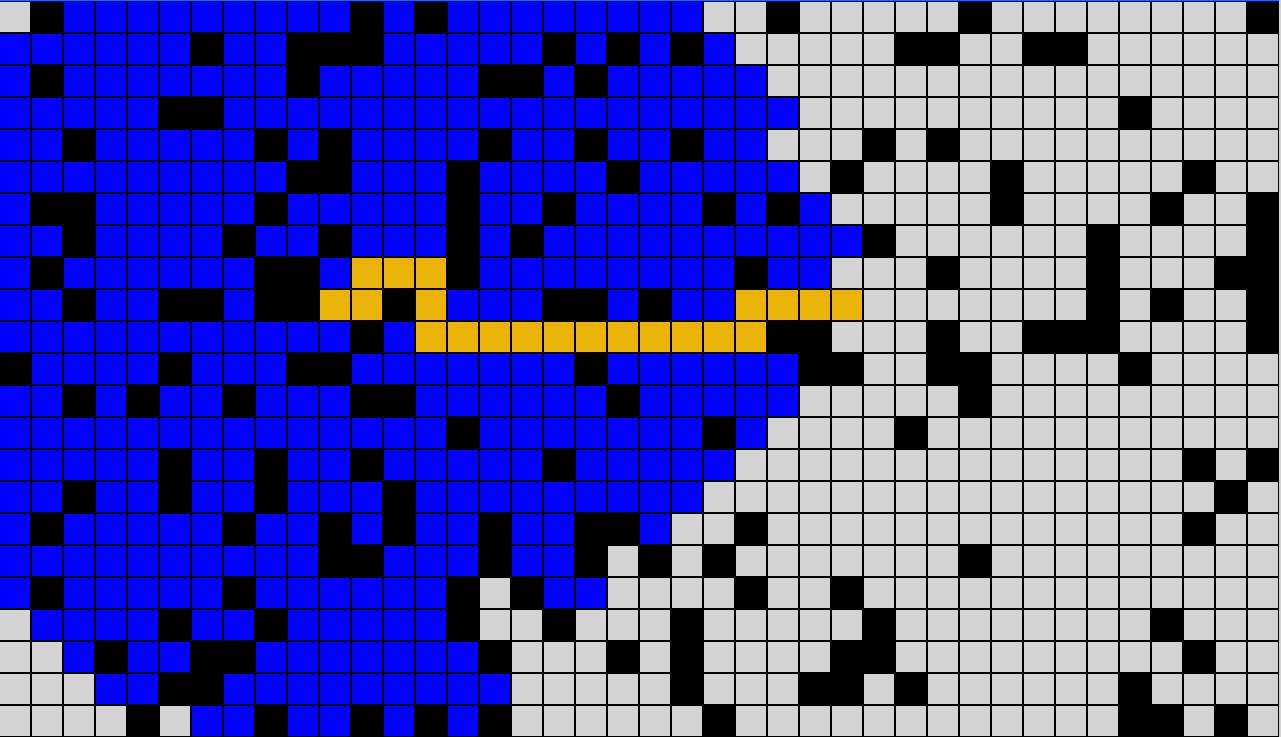
\includegraphics[width=\textwidth]{viz3.png}

\pagebreak
\tableofcontents
\pagebreak

%% Introduktion
\section{Introduktion}
Dijkstra's Algoritme er en kendt algoritme indenfor pathfinding. Formål er at finde den korteste vej fra punkt $a$ til punkt $b$. Dette er en større del af almindelige menneskers liv end man tænker. Hvad er den hurtigste vej til skole eller arbejde? Er det via motorvejen som måske har vejarbejde? Vil det så være hurtigere at tag vejen igennem byen? Disse spørgsmål kan man ofte få hurtigt svar på med ens GPS, som har implementeret diverse pathfinding algoritmer og er tilkoblet internettet med de seneste nyheder om vejarbejde, kø osv. 
\\Jeg vil i denne case med brug af Dijkstra's Algoritme finde sammenhængen mellem den matematiske og programmerings del af rekursion. Rekursion er en stor del af Pathfinding algorithms. Er Dijkstra's Algoritme en god måde at få hjælpe på at finde den korteste vej fra punkt $a$ til punkt $b$.
%% Teori
\section{Teori}

% Hvad er rekursion?
\subsection{Hvad er rekursion?}
Ordet rekursion er en betegnelse for noget som refererer til sig selv. Når noget refererer sig selv betyder det at noget behøver information eller data fra sit forrige jeg. 
Rekursion er oftest betegnet som en rekursionligning i matematik og en som en funktion der kalder sig selv i programmering. 

%Rekursion i Matematik
\subsection{Rekursion i Matematik}
\subsubsection{rekursionligning}
Når der snakkes om rekursion i matematik, snakkes der oftest om en rekursion ligning. 
En rekursion ligning opfattes som en regel der beskriver, hvordan et tal eller element i en talfølge skal beregnes. Hvis vi ser på en simpel talfølge som: {0,1,2,3,4,5...}. Denne talfølge har det næste element i talfølgen altid 1 større end den forrige. Denne talfølge kan dermed beregnes generelt med en rekursion ligning. 
\[x_n = x_{n-1} + 1\] 
Rekursion ligning beregner et vilkårligt element i talfølgen. Dette gøres ved at finde forrige værdi af $n$ med $x_{n-1}$ og derefter gøre $x$ en større. 
Dette eksempelt var meget simpelt da hvad end man vælger $n$ til at være blevet $x$ det samme. 
Et lidt mere kompliceret eksempel af en rekursion ligning er:
\[x_n = 2x_{n-1}\] 
Hvis vi sætter en begyndelsesbetingelse på $x_{0}$.
Med en begyndelsesbetingelse kan der kun komme en talfølge som løsning, 
ud fra eksemplet er talfølgen:
\begin{table}[ht]
  \centering
  \begin{tabular}{ |c|c| }
   \hline
   \textbf{$n$} & \textbf{$x_{n}$}  \\ 
   \hline
   0 & 1  \\
   \hline
   1 & 2 \\ 
   \hline
   2 & 4 \\ 
   \hline
   3 & 8  \\ 
   \hline
   4 & 16  \\ 
   \hline
  \end{tabular}
\end{table}\\
En rekursion ligning kan også have to former, lineær homogen og ikke homogen lineær.\\  
En homogen løsning på en rekursion ligning er hvor en konstant bliver ganget med rekursonslignens $x_{n}$:
\[x_{n}=1,1*x_{n-1}\]
Generel løsninger for en homogen rekursionsligning er at opstille en ligning for at gætte på en løsning.\\ 
\[x_{n}=r*x_{n-1}\]
\[\Longleftrightarrow \]
\[x_{n}=r^n\]
ligningen gælder dog kun for første orden. Orden betyder antal gange du går tilbage i talfølgen.
\begin{center}  
  Første orden \[x_{n}=a_{1}*x_{n-1}\]
  Anden order \[x_{n}=a_{1}*x_{n-1} +a_{2}*x_{n-2}\]
\end{center}
En ikke homogen rekursions ligning er en rekursionsligning hvor en konstant er plusset med $x_{n}$:
\[x_{n}=x_{n}+5\]
Der kan også opskrives en general ligning for en homogen og ikke homogen rekursionsligning af k'et orden:
\begin{center}  
  Homogen rekursionligning af k'et orden \[x_{n}=a_{1}x_{n-1}+a_{2}x_{n-2}\dots a_{k}x_{n-k}\]
  Ikke Homogen rekursionligning af k'et orden \[x_{n}=a_{1}x_{n-1}+a_{2}x_{n-2}\dots a_{k}x_{n-k} + \textbf{f(n)}\]
\end{center}
$f(n)$ er den ikke homogene del af rekursionligningen og er kun en funktion af $n$.
%% Programmering
\subsection{Programmering}
% Rekursion i programmering
\subsubsection{Rekursion i programmering}\label{Rekursion i programmering}
Rekursion i programmering er en funktion som har et rekursivt kald, alså funktion kalder sig selv. Dette kald kan være meget direkte som i eksempel 1 (Simpel rekursions funktion), eller indirekte hvor det ikke er lige så overskuligt at se et rekursivt kald.\footnote{\href{https://www.oreilly.com/library/view/functional-programming-in/9780470971109/xhtml/sec55.html}{Indirect Recursion}}
\begin{lstlisting}[language=JavaScript, caption=Simpel rekursions funktion]
function fractorial(n) {        
  if (n == 1) return 1; 
  else return n*fractorial(n-1) 
} // if n = 4, then exprected output: 24
\end{lstlisting}
Funktionen i eksempel 1 indtag en værdi \textit{n} som parameter. Hvis denne parameteren \textit{n} er 1 stopper det rekursive kald (se linje 2.). Dette betyder også at dette eksempel har et meget direkte grænse hvor \textit{n} ikke kan komme under 1. Linje 3 beskriver så hvordan \textit{n} skal reagere hvis dens værdi ikke er 1. Hvis \textit{n} ikke er 1, men eksempelvis 3 skal den gange nuværende \textit{n} med forrige \textit{n}. I forrige \textit{n} af 3 er 2, derfor skal 2 ganges med dens forrige \textit{n} og således.
\[n(1) = 1 \Leftrightarrow 1\] 
\[n(2) = 2*1 \Leftrightarrow   2\]
\[n(3) = 3*2 \Leftrightarrow   6\]
\[n(4) = 4*6 \Leftrightarrow  \textbf{24}\]

% Varialber
\newpage
\subsubsection{Variabler}
Et variabel er en pladsholder for et stykke data. Typisk set bruger man variabler i brug når man skal gemme et stykke data som man skal bruge forskellige steder i programmet. Disse variabler kan ændres under programmets køretid afhængig i hvordan variables data bliver manipuleret. Variablers data kan eventuelt ændres under programmets køretid, hvis man ønsker. Lidt mere teknisk indeholder et variable særlige set af bits eller af variablenes datatype. Et variable har en datatype som identificere hvilke slags data variabelt kan indeholde. Diverse programmeringssprog bruger dynamiske datatyper, hvor variabler kan indeholde forskellige datatyper. Her et en tabel med forskellige datatyper.
\begin{table}[ht]
  \centering
  \begin{tabular}{ |c|c|c|c| }
   \hline
   \textbf{Datatype} & \textbf{Skrivemåder} & \textbf{Eksempel på data} & \textbf{Kommentar} \\ 
   \hline
   Integer & int & \small{…-3, -2, -1, 0, 1, 2,... 1000} & \shortstack{Kun heltal\\ \footnotesize{(både negativ og positiv)}} \\
   \hline
   Floating Point & float & …, -3.25, -2.11,... 100,12  & \shortstack{Decimaltal\\ \footnotesize{(både negativ og positiv)}} \\ 
   \hline
   String & str eller text & \shortstack{"hello world”, \\ "This is a string"}  &  \shortstack{Et række af karakterer\\ oftest tekst.} \\ 
   \hline
   Array & [ data1,data2,… ] & int val = [-2,-1,0,1,5] & \shortstack{Indeholder en række data \\ under et navn} \\ 
   \hline
   Character & char & @, s, ¤, k…  & Kun et symbol \\ 
   \hline
   Boolean & bool & True (1) eller False (0)  & Enten sandt eller falsk \\ 
   \hline
   Constant & const & "Hello", -3, 22, [1, 2, 3] & \shortstack{Dynamisk datatype, \\ men konstant værdi} \\ 
   \hline
  \end{tabular}
\end{table}

%Objekter

\subsubsection{Objekter}
Et objekt er en abstrakt enhed med specifikke karakteriseringer og opførelse. Et objekt kan være et variable, datastruktur, en funktion eller en kombination alle dem alle. Et praktiskt eksempl på dette kan være en bil som objekt. En bil har specifikke karakteriseringer såsom hjul, farve, producent osv. En bil har også opførsel som at starte motoren, accelerere bilen m.m.\footnote{\href{https://techterms.com/definition/object}{Objekter}} 
\\Hvis vi tager samme praktiske eksempel på en bil som objekt, kan vi overføre det til kode med en “Klasse” som er en form for plan over alle klassens objekter
\begin{lstlisting}[language=Java, caption=Eksempel på et objekt]
  class Car { // Blueprint a car
   int model;
   int year;
   string color;
   
    void drive() { // objekt
      // Get the car to drive
    }

    void reverse() { // objekt
      // Get the car to reverse
    }
}
\end{lstlisting}
%Arrays
\subsubsection{Arrays}
Et array er en datastruktur, der indeholder en gruppe af elementer. Disse elementer er typisk alle af samme datatype, såsom et integer eller en string. Arrays bruges typisk set i computerprogrammer til at organisere data, så et relateret sæt værdier nemt kan sorteres eller søges.
\begin{lstlisting}[language=JavaScript, caption=Eksempel på et array]
  // Array with constant values of datatype String
  const cars = ["Audi", "Volvo", "BMW"];
  cars[0] = "Audi" // Index 0 of array
\end{lstlisting}

% Løkker
\subsubsection{Løkker}
En løkke er et stykke kode som vil fortsætte med at køre indtil en given betingelse er opfyldt. der er to slags løkker, “while” - løkker og “for”-løkker. “While” løkker kører ind til betingelsen i parentesen bliver opfyldt. Mens “for” løkker lavet selv et variabel, som i det simpleste tilfælde vil tælle op eller ned fra og køre det antal gange ifølge betingelse. Løkker er meget brugbare siden det stopper en fra at skulle skrive mange linjer af den samme kode hvis man skal køre noget flere gange.
\begin{lstlisting}[language=JavaScript, caption=Eksempel på et for løkke]
for (let i = 0; i < 5; i++) {
  console.log(i);
} // exprected output: 0,1,2,3,4
\end{lstlisting}

% Betinget udførelse
\subsubsection{Betinget udførelse (if statement)}
Betinget udførelse eller “if statement”, er et stykke kode som checker om en betingelse opfyldt nogle specifikke kriterier. Hvis de betingelser bliver opfyldt vil koden inde i dette if statement blive kørt. Med et if statement kan man give den flere kriterier ved at lave en “else if” eller “else” statement efter den første stykke kode. “else if” er et til if statement med en betingelse før den bliver kørt, samtidig med at dette stykke kode kun bliver kørt hvis det første if statement ikke opfylder sin betingelse. Et “else” statement er bare et stykke kode som vil blive kørt hvis koden ikke opfyldte sin betingelse.
\begin{lstlisting}[language=JavaScript, caption=Eksempel på betinget udførelse]
let val = 5; 

if(val == 1){
  console.log("The value is now 1!");
}else console.log("The value is not 1"); // exprected execution of statement
\end{lstlisting}
\subsubsection{Dijkstra's algoritme}
Dijkstra’s algoritme består af Breadth-First Search Algorithm (BFS) med et lille twist. BFS er designet til at søge igennem et data tree eller en graf struktur. BFS algoritmen søger først alle “neighbors” til et givne “node” før den søge i naboernes “children”. Twistet i Dijkstra's algoritme er dog Dijkstra gøre brug af en prioriterings kø af “nodes”, for at prioritere hvilke naboer Dijkstra’s skal søge igennem først.\footnote{\href{https://www.baeldung.com/cs/graph-algorithms-bfs-dijkstra}{Breadth-First Search in Dijkstra}} 
\\“Node” indenfor programmering er datapunkter i et data tree eller en anden form for datastruktur. “Neighbors” eller naboer er nodes som har direkte kommunikation for den første node. “Children” er så tredje leds nodes til første node.\footnote{\href{https://www.freecodecamp.org/news/all-you-need-to-know-about-tree-data-structures-bceacb85490c/}{Everything about datatrees}} 
\begin{figure}[ht]\label{gennemgang af datatree}
  \centering
  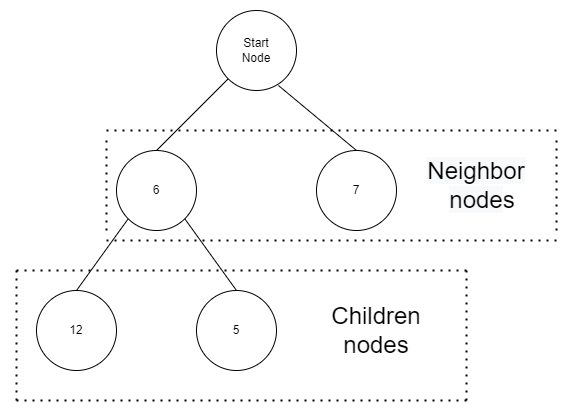
\includegraphics[width=0.80\textwidth]{img/nodeSetup.png}
  \caption{Illustration af et datatree med Nodes}
\end{figure}
\newpage
\begin{wrapfigure}{r}{0.40\textwidth} %this figure will be at the right 
  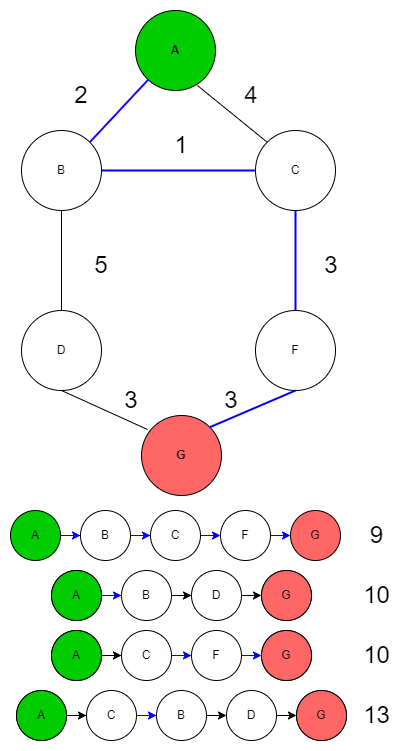
\includegraphics[width=0.4\textwidth, height=0.417\textheight]{img/AlgoViz.png}
  \caption{Eksempel på gennemgang af datatree af Dijkstra’s Algorithm}\label{eksempel af datatree}
  \centering
\end{wrapfigure}

Dijkstra’s algoritme er designet til at finde den korteste vej mellem 2 notes. Algorithmen søger og finder diverse veje med den korteste vej og beregner den korteste vej gennem hver node som ikke er søgt igennem. Derefter opdatere den nabo nodernes med den korteste vej imens den holder øje med hvilke nodes algoritmen allerede har søgt igennem. Vejen til hver node har en "vægt". En vægt betyder sværhedsgraden for at kommer til valgte node. Et praktisk eksempel på dette kunne være transport. En højere vægt værdi kan være på grund af eventuelt vejarbejde, kø osv. Figur \ref{eksempel af datatree} har også lignende vægte bare data raleterende.
\\Eksemplet her viser en datatree med følgende nodes $A,B,C,D,F,G$. Algoritmen skal finde den korteste vej fra node $A \rightarrow G$. Algorithmen vil først søge igennem nabo nodes til vores start node A. Vejen fra node $A \rightarrow B$ koster 2 og vejen fra $A \rightarrow C$ koster 4. Derfor indtil videre er den korteste vej B. Så søger algorithmen fra node $B \rightarrow C$ og D, vejen til C koster nu kun 3 ud fra forrige $A \rightarrow C$. Så søges vejen fra $C \rightarrow F$, og den er kortere end $B \rightarrow D$ som kostet 5. Til sidst søges den korteste vej fra $F \rightarrow G$ og $D \rightarrow G$, som vejen $F \rightarrow G$ er stadig den korteste vej. Dermed bliver den korteste vej $A \rightarrow B \rightarrow C \rightarrow F \rightarrow G$ med total vægtkost på 9. 

\subsubsection{Dijkstra’s Algorithm Pseudocode}
Nu når vi ved hvordan Dijkstra’s Algorithm virker skal vi prøve så oversætte det til kode.
Den bedste måde at generelt oversætte algoritmen kan vi lave en Pseudokode. En Pseudokode er en måde at skrive en algoritme eller en processen på en general programmerings måde uden at implementere direkte kode. Dette kan være hjælpe andre med generelt at forstå en algoritme kodemæssigt.\footnote{\href{https://www.programiz.com/dsa/dijkstra-algorithm}{Dijkstra Algorithm Pseudokode}}
\begin{lstlisting}[language=JavaScript, caption=Dijkstra’s Algorithm Pseudocode teoritisk (på Engelsk)]
function dijkstra(G, S)
for each vertex V in G
    distance[V] // infinite
    previous[V] // NULL
    If V != S, add V to Priority Queue Q
distance[S] // 0

while Q IS NOT EMPTY
    U // Extract MIN from Q
    for each unvisited neighbour V of U
        tempDistance // distance[U] + edge_weight(U, V)
        if tempDistance < distance[V]
            distance[V] // tempDistance
            previous[V] // U
return distance[], previous[]
\end{lstlisting}
For nemmer forståelse har jeg selv oversat Pseudokoden til Dansk:
\begin{lstlisting}[language=JavaScript, caption=Dijkstra’s Algorithm Pseudocode oversat til Dansk]
function Dijkstra(G, S); // G = Graf, S = Source (evt. startpunkt)
  for hver V i G // V = vej
    afstand[V] = infinity // set alle veje til infinity
    forrige[V] = null
    hvis V != S
      V += Q // Q = prioriterings queue (gem)
  afstand[S] // afstand fra node til node

  imens Q er tom
      U // U = min value fra Q
      for hver nabo V af U som stadig i Q
        midlertidigAfstand  // afstabd[U] + G.Sider[U, V]
        hvis midlertidigAfstand < afstand[V]
          afstand[V] // midlertidigAfstand
          forrige[V] // U

return afstand[], forrige[]
\end{lstlisting}
  

\newpage
\section{Metode og Analyse}
At bruge Dijkstra's algoritme til at finde den korteste var fra $a$ til $b$, er på papir en effektiv måde at gøre det på. Men er det dog også sådan i praksis? Hvilke scenarier er Dijkstra's algoritme god imod andre pathfinding algoritmer såsom A* search algorithmen? 
\subsection{Dijkstra mod andre algoritmer}
Dijkstra er en af de mest kendte algoritmer indenfor pathfinding. 
Der er andre pathfinding algorithms som bygger videre på Dijkstra’s algoritme, 
som er bedre til at løse andre problemer end Dijkstra. En af efterkommerne af Dijkstra’s algorithm er A* 
(udtalt A star). A* er en generelt mere effektiv algoritme i forhold til Dijkstra’s, 
dette er fordi A* hænger tungt på “heuristic”. Heuristic (eller heuristik på dansk) inde for programmering, 
er en designet teknik til at løse et problem hurtigere. Man kan se det som en form for systematisk søgning 
efter information eller afprøvning af de bedste muligheder.\footnote{\href{https://softjourn.com/insights/heuristic-programming}{Heuristic Programming}} Det der også gøre A* algoritmen hurtigere 
og bedre i de fleste tilfælde er at den er en informeret algoritme. Dette betyder at A* har mulighed for lidt 
mere infomation på grund af dens brug af Heuristics. Dijkstra’s har ikke denne fordel, som A* har \footnote{\href{https://stackabuse.com/dijkstras-algorithm-vs-a-algorithm/}{Dijkstra's Algorithm vs A* Algorithm}}. Dijkstra’s 
er en form for et “brute force” på et problem, da den bare søger løs for slut noden. 
Ordet “brute force” betyder at algorithmen løser et problem den mest simple måde, dette er ofte mindre elegant og en langsom måde at løse problemer på. 
Dette eksempel viser et eksempel på Dijkstra’s algoritme og A* 
search og hvordan de hver især løser en labyrint.  
\begin{figure}[ht]
  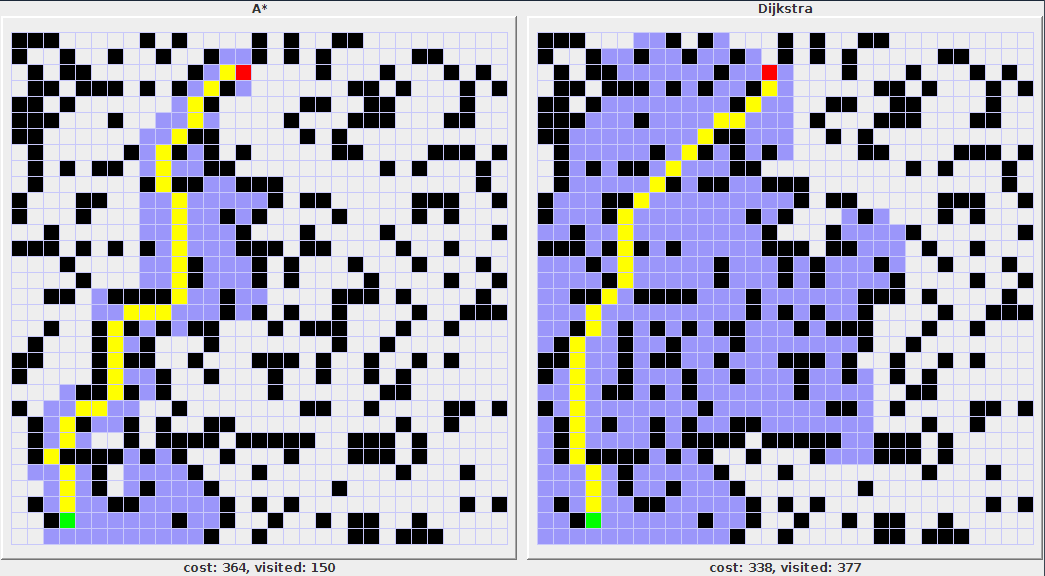
\includegraphics[width=\textwidth]{AstarvsDjikstra.png}
  \caption{A* search vs. Dijkstra algoritme}\label{A*vsDjikstra}
\end{figure}\footnote{Kevin Wang - \href{http://plainaslife.blogspot.com/2015/02/compare-with-dijkstra-algorithm.html}{Compare A* with Dijkstra algorithm}}
\\Figur \ref{A*vsDjikstra} viser et godt eksempel på hvordan A* har haft en bedre fornemmelse for hvor slut noden er på grund af dens brug af Heuristics. A* har meget færre besøgte nodes (blå celler i labyrinten) som har øget dens hastighed i at løse problemet. 
Hvor imod Dijkstra har over dobbelt så mange besøgte nodes som den skulle gå igennem. 
\newpage
\subsection{Gennemgang i min kode}
Første step til at gennemgå funktionen Dijkstra’s algoritme (\ref{lst:Dijkstra}), er at den indtager 3 parameter. parametere er “grid”, 
“startNode” og “Finishnode”. Disse parameter bliver brugt til diverse ting i algorithmen. “grid” bruges til at indsamle alle “unvisitedNodes” nodes fra griddet. 
“StartNode” bruges til at definere hvor algoritmen skal starte, og selfølig “Finishnode” til at definere hvor vi skal slutte. Bemærk at algoritmen ved ikke på forhånd hvor “FinishNode” er, algoritmen skal blot bruge den til at se om det har fundet “FinishNode”.   
\begin{lstlisting}[language=JavaScript]
function dijkstra(grid , startNode , finishNode)
\end{lstlisting}
Algorithmen sortere så alle nodes i griddet ud fra deres afstand fra hinanden, til at finde de tætteste nodes på “startNode”. Disse nodes bliver så defineret i variablet “closestNode”.
\begin{lstlisting}[language=JavaScript]
sortNodesByDistance(unvisitedNodes);
const closestNode = unvisitedNodes.shift();
\end{lstlisting}
Nu begynder diverse betingelser at blive tjekket igennem for den “closestNode”. Den “closestNode” bliver først tjekket for om den er en væg, hvis det er springer den node over. Derefter tjekket om vi sidder fast og der ikke er nogen løsning. Dette sker ved at se om alle resterende nodes vi kan få fat i, har deres oprindelig startværdi “Infinity".
\begin{lstlisting}[language=JavaScript]
if (closestNode.isWall) continue; // If we encounter a wall , we skip it.

// If the closest nodes distance = infinity, then we are trapped
// and should stop.
if (closestNode.distance === Infinity) return visitedNodesInOrder; 
\end{lstlisting}
Når alle betingelserne er opfyldt sætter vi så det tætteste node “closestNode” til besøgt og tilføjer den til vores prioriterings kø. 
\begin{lstlisting}[language=JavaScript]
// If node passed parameters, then visited
  closestNode.isVisited = true;
// Push node to priority queue
  visitedNodesInOrder.push(closestNode);
\end{lstlisting}
Hvis vi så er så heldige at finde vores mål “FinishNode” stopper vi så søgningen og returnere vores resultater. Ellers hvis vi ikke finder vores mål, opdatere vi bare vores nye grid med vores “closestNode” som besøgt. 
\begin{lstlisting}[language=JavaScript]
// If reached finishNode, return visitedNodesInOrder for furthere use.
  if (closestNode === finishNode) return visitedNodesInOrder;
// Update grid with new visited nodes
  updateUnvisitedNeighbors(closestNode , grid);
\end{lstlisting}
\subsubsection{Rekursion i min kode}
Som nævnt \ref{Rekursion i programmering} kan det rekursive kald i en funktion være direkte og indirekte. 
Det rekursive kald i mit tilfælde er indirekte og kan være svær at gennemskue. \\
Min kode for Dijkstra’s Algoritme (\ref{lst:Dijkstra}) er opbygget på, at den starter med indsamle alle nodes 
fra griddet. Alle nodes bliver opsamlet i et array "unvisitedNodes" fra ekstern funktion getAllNodes (\ref{lst:getAllNodes}). Dermed er der allerede et loft på funktionen, 
dette loft vil så stoppe det rekursive kald, hvis der ikke er flere nodes tilbage i griddet:
\begin{lstlisting}[language=JavaScript]
const unvisitedNodes = getAllNodes(grid); // get nodes from grid
\end{lstlisting}
Dette er ligesom linje 2 i \ref{Rekursion i programmering}, her stopper det rekursive kalde også: 
\begin{lstlisting}[language=JavaScript]
if (n == 1) return 1;
\end{lstlisting}
Det rekursive kald kommer via et while loop (linje 5 i \ref{lst:Dijkstra}). 
Dette while loop brydes kun, hvis alle “unvisitedNodes” har en længde (altså blevet søgt igennem). 
\begin{lstlisting}[language=JavaScript]
while (!!unvisitedNodes.length) // caster unvisitedNodes til boolean
\end{lstlisting}
\subsubsection{Dijkstra’s Algoritme visualiseret}
Det er godt første skridt at implementere Dijkstra's algoritme til et grid med diverse nodes. Det er bare mere interessant at se det visualiseret. Jeg har opbygget et grid som minder lidt om Kevin Wangs grid (\ref{A*vsDjikstra}) , jeg har dog kun implementeret Dijkstra’s algoritme. Med min lille visualisering af Dijkstra’s algoritme kan man se hvordan algoritmen opføre sig i et givende miljø som man selv kan lave eller tilfældig gøre. \\
Bemærk jeg har valgt at referere til min egen kode på \href{https://github.com/}{Github.com} som kilde. Dette er gjort for at undgå store mængde bilag med kode, der ikke har så stor betydning for denne case.\footnote{Min visualisering af \href{https://github.com/johannes67890/Pathfinding.git}{Dijkstra’s Algoritme}}     
\begin{figure}[ht]%
  \centering
  \subfloat[\centering Visualisering af Dijkstra der søger efter sit mål]{{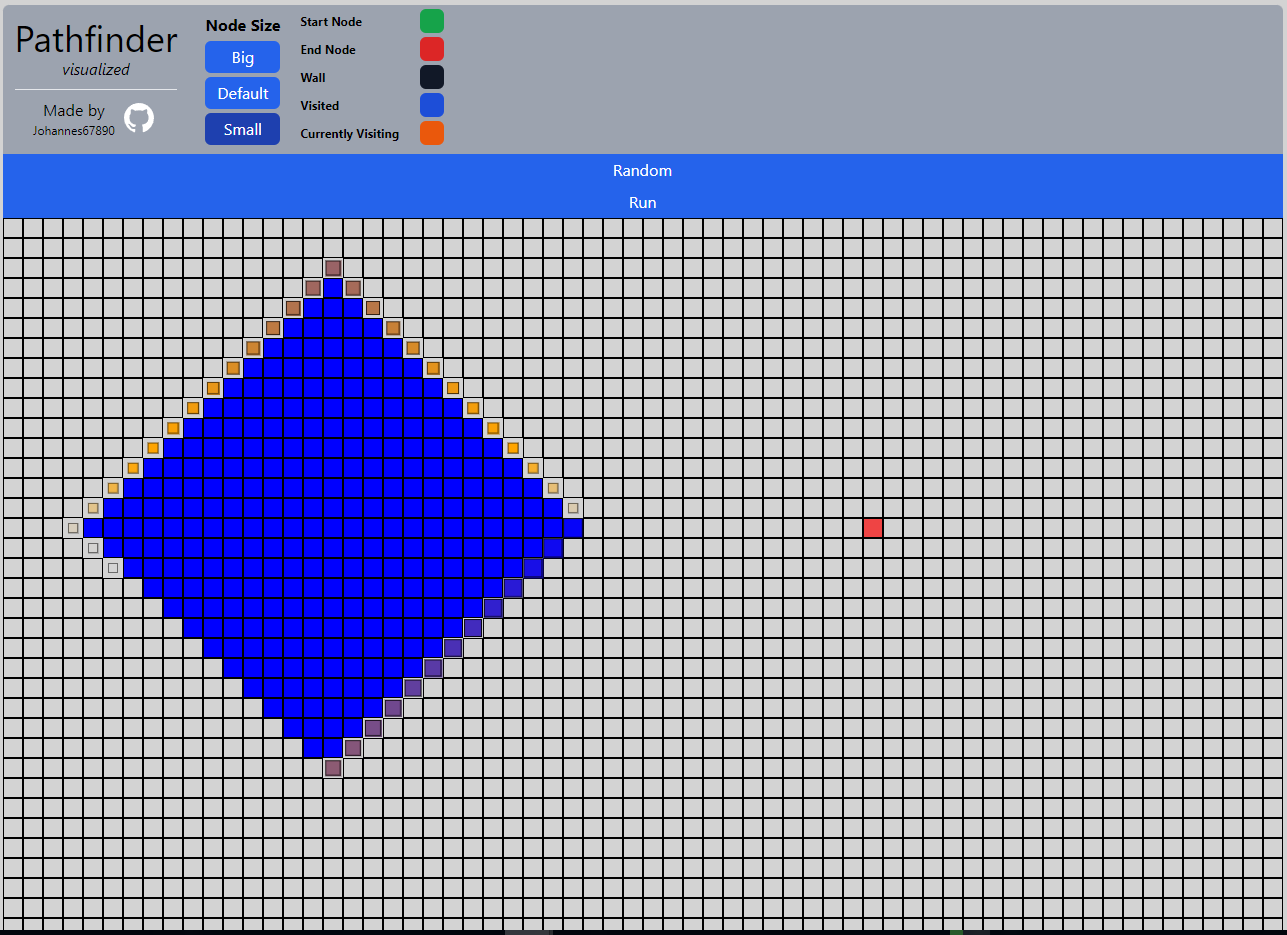
\includegraphics[width=9cm]{viz1.png} }}%
  \subfloat[\centering Visualisering af Dijkstra der har fundet sit mål]{{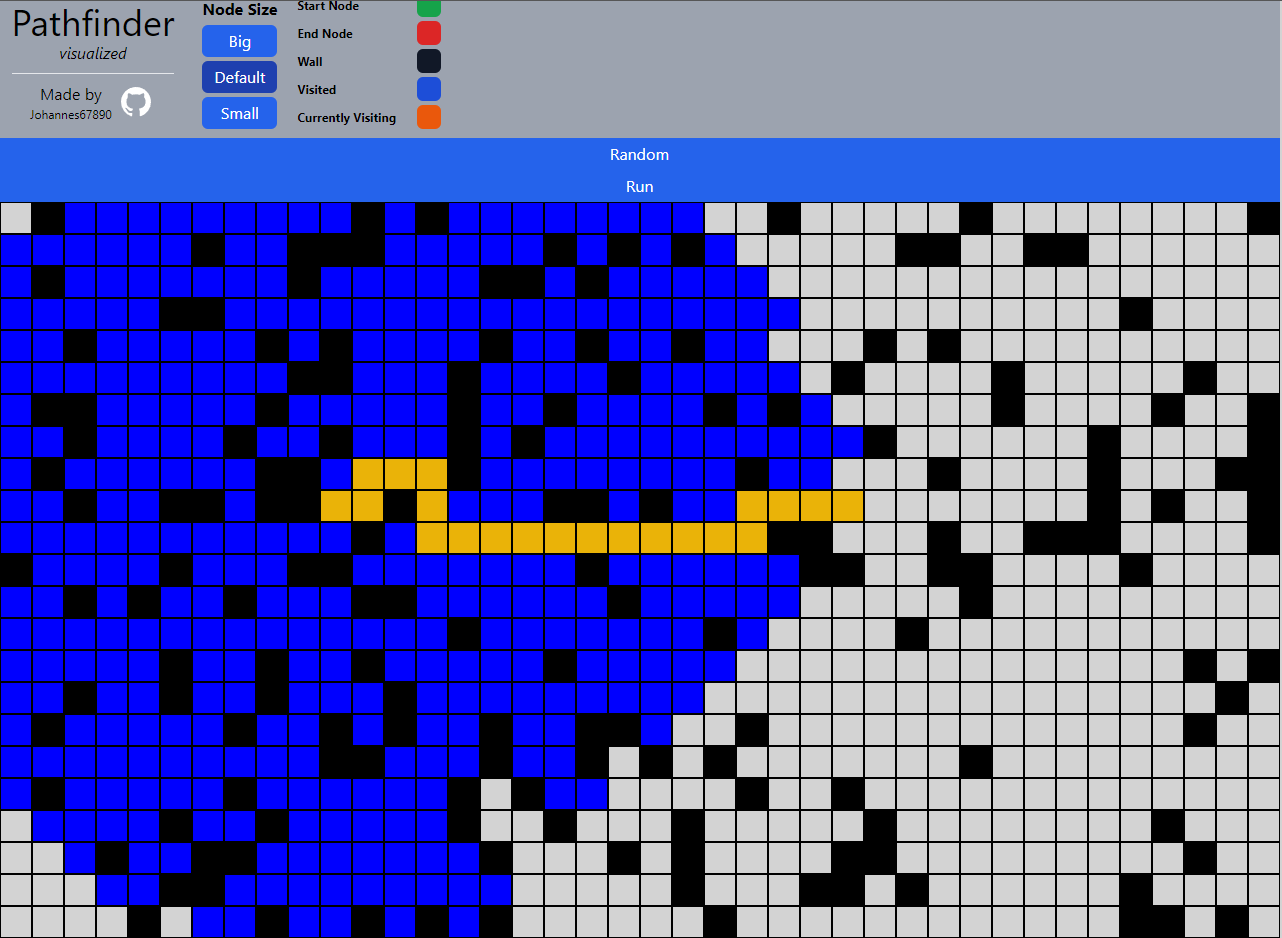
\includegraphics[width=9cm]{viz2.png} }}%
  \caption{2 Screenshots af min Visualisering af Dijkstra’s Algoritme}%
\end{figure}
\section{Konklution}
Der er mange forskelige måder at kommer fra $a$ til $b$. Det er ikke så simpelt som man måske skulle tro, selvom man har en algoritme til at gøre det for en. Det kommer meget an på problemet som ligger foran en. Er det et problem hvor man har mulighed for at bruge A* algorithmen og gøre brug af dens Heuristic? Eller skal man bare holde sig til Dijkstra som brute forcer problemet. Det er en større diskussion om hvilken algoritme som passer bedst til hvad. Dog er Dijkstra en okay måde at løse pathfinding også selvom den ikke er helt så optimal til de fleres scenarier i data trees og grafer. Dijkstra’s algoritme kan skrives på forskellige måde, både i form af dens brug og om algoritmen har et direkte eller indirekte rekursivt kald.   
\newpage
\section{Litteraturliste}
Dijkstra's Algorithm. (s.d.). I: Programiz. \\Lokaliseret den 25. Febuar 2022 på \href{https://www.programiz.com/dsa/dijkstra-algorithm}{https://www.programiz.com/dsa/dijkstra-algorithm}\\

Heuristic Programming. (s.d.). softjourn. \\Lokaliseret den 25. Febuar 2022 på \href{https://softjourn.com/insights/heuristic-programming}{https://softjourn.com/insights/heuristic-programming}\\

Indirect Recursion. (s.d.). Oreilly. \\Lokaliseret den 25. Febuar 2022 på \href{https://www.oreilly.com/library/view/functional-programming-in/9780470971109/xhtml/sec55.html}{https://www.oreilly.com/library/view/functional-programming-in/9780470971109/xhtml/sec55.html}\\

Jørgensen, Johannes. (s.d.). Pathfinding: Min visualisering på Djikstra's Algoritme. \\github. Lokaliseret den 25. Febuar på \href{https://github.com/johannes67890/Pathfinding}{https://github.com/johannes67890/Pathfinding}\\

Kevin Wang, K, W. (2015, 28. Febuar). Plain As Life. plainaslife. \\Lokaliseret den 25. Febuar 2022 på \href{http://plainaslife.blogspot.com/2015/02/compare-with-dijkstra-algorithm.html}{http://plainaslife.blogspot.com/2015/02/compare-with-dijkstra-algorithm.html}\\

Mila Lukic, M, L. (2021, 10. December). Dijkstra's Algorithm vs A* Algorithm. Stackabuse. \\Lokaliseret den 25. Febuar 2022 på \href{https://stackabuse.com/dijkstras-algorithm-vs-a-algorithm/}{https://stackabuse.com/dijkstras-algorithm-vs-a-algorithm/}\\

Object. (2019, 28. Febuar). TectTerms. \\Lokaliseret den 25. Febuar 2022 på \href{https://techterms.com/definition/object}{https://techterms.com/definition/object}\\

Said Sryheni, S,S. (2021, 25. August). Difference Between BFS and Dijkstra’s Algorithms.\\ Baeldung. Lokaliseret den 25. Febuar 2022 på \href{https://www.baeldung.com/cs/graph-algorithms-bfs-dijkstra}{https://www.baeldung.com/cs/graph-algorithms-bfs-dijkstra}\\

TK. (s.d.). Everything you need to know about tree data structures. FreeCodeCamp. \\Lokaliseret den 25. Febuar 2022 på \href{https://www.freecodecamp.org/news/all-you-need-to-know-about-tree-data-structures-bceacb85490c/}{https://www.freecodecamp.org/news/all-you-need-to-know-about-tree-data-structures-bceacb85490c/}\\



\newpage
\section{Bilag}
% dijkstra algo
\subsection{Kode}
Kode inspirret af \href{https://github.com/clementmihailescu/Pathfinding-Visualizer-Tutorial}{clementmihailescu}'s Pathfinding-Visualizer
\begin{lstlisting}[language=JavaScript, caption=Kode for Dijkstra's Algoritme, label={lst:Dijkstra}]
function dijkstra(grid, startNode, finishNode) {
  const visitedNodesInOrder = [];
  startNode.distance = 0;
  const unvisitedNodes = getAllCells(grid); // get cells from grid
  while (!!unvisitedNodes.length) {
    sortNodesByDistance(unvisitedNodes);
    const closestNode = unvisitedNodes.shift();

    if (closestNode != undefined) {
      // If we encounter a wall, we skip it.
      if (closestNode.isWall) continue;
      // If the closest nodes distance = infinity, then we are trapped 
      // and should stop.
      if (closestNode.distance === Infinity) return visitedNodesInOrder;
      // If node passed parameters, then visited
      closestNode.isVisited = true; 
      // Push node to priority queue
      visitedNodesInOrder.push(closestNode);
      // If reached finishNode, return visitedNodesInOrder for furthere use.
      if (closestNode === finishNode) return visitedNodesInOrder;
      // Update grid with new visited nodes
      updateUnvisitedNeighbors(closestNode, grid); 
    } else console.log("error, closestNode returned 0");
  }
}
\end{lstlisting}
\begin{lstlisting}[language=JavaScript, caption=Kode for opdatering af unvisitedNodes]
function updateUnvisitedNeighbors(node, grid) {
const unvisitedNeighbors = getUnvisitedNeighbors(node, grid);
for (const neighbor of unvisitedNeighbors) {
  // set node from infinity to 1 (now visited).
  neighbor.distance = node.distance + 1;
  neighbor.previousNode = node; // set new node to previous node
  }
}
\end{lstlisting}
\begin{lstlisting}[language=JavaScript, caption=Kode for finde tætteste nodes]
  function sortNodesByDistance(unvisitedNodes) {
  unvisitedNodes.sort(
    (nodeA, nodeB) => nodeA.distance - nodeB.distance
  );
}
\end{lstlisting}
\begin{lstlisting}[language=JavaScript, caption=Kode for at søge nye nodes]
  function getUnvisitedNeighbors(node, grid) {
    const neighbors = [];
    const { col, row } = node;
    if (row > 0) neighbors.push(grid[row - 1][col]);
    if (row < grid.length - 1) neighbors.push(grid[row + 1][col]);
    if (col > 0) neighbors.push(grid[row][col - 1]);
    if (col < grid[0].length - 1) neighbors.push(grid[row][col + 1]);
    return neighbors.filter((neighbor) => !neighbor.isVisited);
  }
  
\end{lstlisting}
\begin{lstlisting}[language=JavaScript, caption=Kode for finde korteste vej]
  function getNodesInShortestPathOrder(finishNode) {
  const NodesInShortestPathOrder = [];
  let currentNode = finishNode;
  while (currentNode !== null) {
    NodesInShortestPathOrder.unshift(currentNode); //shift back though finishNode
    currentNode = currentNode.previousNode;
  }
  console.log("Shorstes path length: ", NodesInShortestPathOrder.length);

  return NodesInShortestPathOrder;
}
\end{lstlisting}
\begin{lstlisting}[language=JavaScript, caption=Kode for finde alle nodes i grid, label={lst:getAllNodes}]
function getAllNodes(grid) {
  const Nodes = [];
  for (const row of grid) {
    for (const node of row) {
      Nodes.push(node);
    }
  }
  return Nodes;
}
\end{lstlisting}
\newpage
\subsection{Screenshots af mit program}

\begin{figure}[ht]%
  \centering
  \subfloat[\centering Visualisering af Dijkstra der søger efter sit mål]{{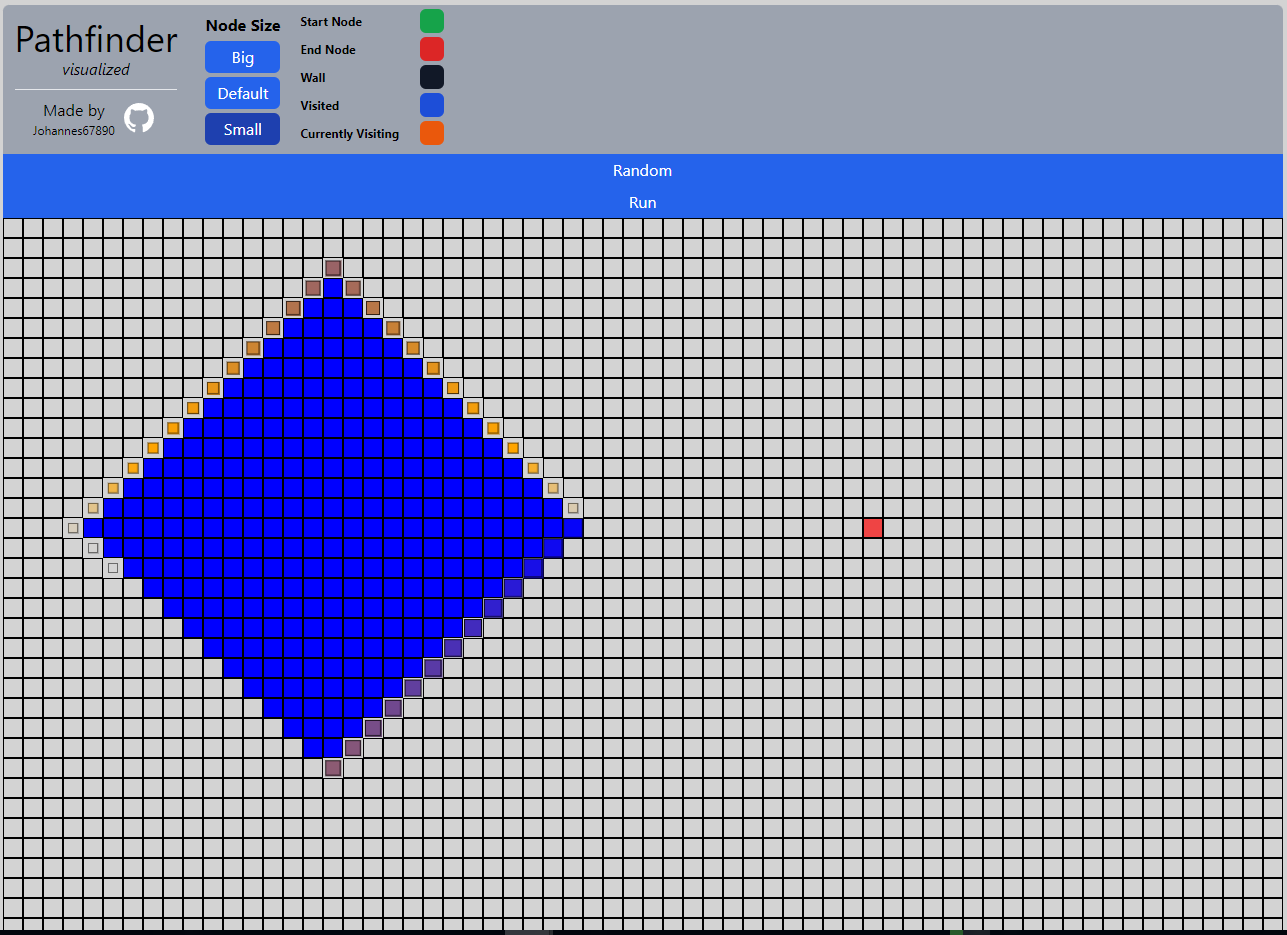
\includegraphics[width=0.73\textwidth]{viz1.png} }}%
  \qquad
  \subfloat[\centering Visualisering af Dijkstra der har fundet sit mål]{{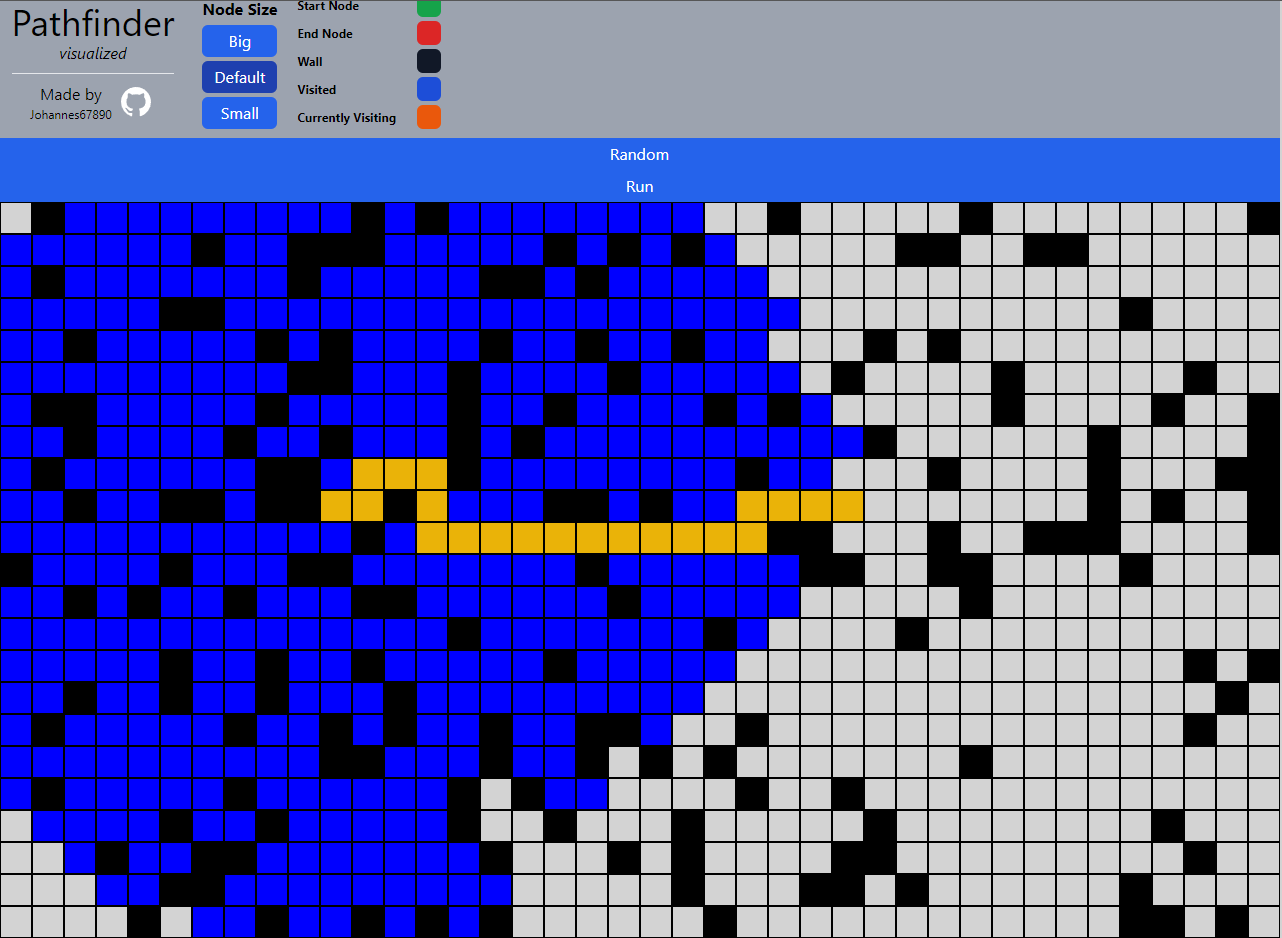
\includegraphics[width=0.73\textwidth]{viz2.png} }}%
  \label{fig:Vizualication}%
\end{figure}

% https://i.gyazo.com/0b387356445aefc069204298e796aff7.mp4 
\end{document}